\chapter{Contributions from ASEAN partners} \label{abstracts}

\tab After the project wrap-up workshop in Jakarta (cf. \ref{ws_jakarta}), participants were asked to provide an abstract summarizing prominent challenges and solutions for their home countries. It encompasses various issues such as remote sensing or disaster risk reduction.

\vspace{0.4 cm}

The abstract presented below are sorted in the alphabetical order of countries and reproduced exactly as received.

\section{Indonesia (1/2)}

\vspace{0.5 cm}

{
	\begin{center}
	{\large \bfseries The used of satellite data for identifying potential fishing ground in Indonesia Seas\par}
	\vspace{0.5 cm}
	{\bfseries I Nyoman Radiarta, Teja Arief Wibawa, Rizky Hanintyo, Komang Iwan Suniada\par}
	{\itshape Institute for Marine Research and Observation (IMRO)\par}
	{\itshape Jalan Baru Perancak, Negara Jembrana-Bali 82251\par}
	{\itshape Email: radiarta@kkp.go.id; radiarta@gmail.com\par}
	\end{center}
	{\tab High quality data of marine environmental plays an important role on resources management. Indonesia with large marine areas need to be manage in proper way in order to support sustainable use of marine and coastal resources. The used of satellite data with low cost is high demanding for operational fisheries oceanography in Indonesia Seas. Several studies on the use of satellite data have shown valuable results for fisheries management. Various satellite remote sensing data has provided real data which can be used to monitor marine resources. The command uses of satellite data including MODIS (Aqua and Terra), SeaWiFs, NOAA, ASTER, and Landsat. The present paper gives an overview of the application of satellite remotely sensed data for identifying potential fishing ground (PFG) around the Indonesia Seas. Remotely sensed data used as primary data to analyst the PFG maps, such as sea surface temperature, sea surface chlorophyll-a, front, and PAR data. The PFG maps was semi-automatic processed, combining between computer and human processes. The PFG maps have three different products namely: national PFG, harbor PFG and specific area PFG. The PFG maps were distributed routinely through several sources: website, facsimile, and mobile applications ("NELPIN= nelayan pintar"). PFG maps were validated by using several approach, such as research activities and feedback from local government/users, overlay fishing vessel from radar detection, and overlay VIIRS data. Using the radar technology (identification of fishing vessel), we were able to validate the PFG maps. As an example in this paper, we attempt to analyst and overlay the PFG maps and distribution of fishing vessel in Natuna Sea (Fisheries Management Area/FMA-711). We found that the accuracy of the PFG maps were variable with the average accuracy about 40\%. In addition we were also conducted validation using VIIRS (night time images) data. From this application shows that low cost satellite data has become an ideal tool for identifying potential fishing ground. This results show that the enhancement of PFG maps are still need to be considered in order to support the operational fisheries, The enhancement the PFG maps through process for automatic systems and increase their accuracy are highly required.\par}
\begin{center}
\textbf{Keywords:} satellite data, fisheries oceanography, potential fishing ground, Indonesia Seas. \par
\end{center}
}


\section{Indonesia (2/2)}

\vspace{0.5 cm}

{
	\begin{center}
	{\large \bfseries Satellite Remote Sensing Application for Economic Development in Indonesia\par}
	\vspace{0.5 cm}
	{\bfseries M. Rokhis Khomarudin\par}
	{\itshape Remote Sensing Application Center, LAPAN, Indonesia\par}
	{\itshape Email: Rokhis.Khomarudin@lapan.go.id\par}
	\end{center}
	{\tab Why is remote sensing necessary in Indonesia? Indonesia is a large country with 1,879,183 km2 of lands and 3,544,743 km2 of oceans.  Without remote sensing, Indonesia will have some difficulties in monitoring the country. Since 2013, Indonesia has Space Act No. 21/2013 which give some mandates to LAPAN. The mandates are providing remote sensing data with minimum cloud coverage and providing the standard methodology for remote sensing data processing and analyzing.  Due to this reasons, LAPAN developed three ground stations to receive remote sensing data. They are located in Parepare (South Sulawesi), Rumpin (West Java), and Pekayon (Jakarta). With this three ground stations, it can cover all Indonesian area and receive low-resolution data (Terra/Aqua MODIS, NOAA, Suomi NPP, and Himawari-8), medium-resolution data (Landsat-7 and Landsat-8) and high-resolution data (SPOT 6/7). These data are available free for the government institutions. Other data that provided by LAPAN are very high-resolution data such as Pleiades,  Quickbird, Worldview, and some SAR imageries.  To serve users, not only receive the remote sensing data, LAPAN also provides the cloud free mosaic data of Landsat-8. It is now available from 1999 to 2016. It is useful for land use mapping with maximum scale 1: 100,000. It is also useful for forest change and degradations.
	
What is related to the economic development? What applications that have been done in Indonesia? The remote sensing technology has been applied in many sectors, but it can be divided into five categories, (1) land resources, (2) coastal and marine resources, (3) environment, (4) disaster mitigation, and (5) other strategic application.  Agriculture, forestry, mining, regional planning, and water resources are in the land resources category. Potential fishing ground, mangrove, coral reefs, and water quality are in the coastal and marine resources. Hazardous waste, deforestation, land use change, and oil spills are in the environment categories. Flood, Landslide, volcano eruptions, forest fires and drought detection and monitoring are in the disaster mitigation category. Tax, drag planting, and security assessment are in the other strategic applications. All those applications have been done in the remote sensing applications center of LAPAN.  In relation to the economic development in Indonesia, there are several applications have been done and support the ministries. The monitoring of paddy growth every 8-days can be used in estimating the paddy production, decision to import rice from other countries, and decision of fertilizer and farmer machine distributions. The potential fishing ground can be used to increase the number of catching fish and the efficiency of oil. With this information. The application of tax, the remote sensing can be used to increase the number of taxes that have to be paid by the taxpayers, especially for plantations, mining, and forestry companies. These applications have to improve in the other provinces to increase the tax payments. Another application which can support the economic development is the mining areas identification. It can help the government or mining company to identify the location of mining areas. It will increase the number of mining exploitation and also increase the country incomes. 
LAPAN provide the remote sensing data and also provide many applications to support the economic development. The next question is "What are the challenges? How to convince users?" This paper answer this two questions. The first challenge is the second question, it is convincing users. To convince the user, the remote sensing application should be accurate and also up-to-date. The accuracy can be served by good research and the up-to-date information can be served by high-temporal-resolution of remote sensing data and also the automatic image processing. The research collaborations with the users are necessary, I will meet the requirements of users. LAPAN has collaborations with many government institutions, local government, private companies, and also foreign institutions. This will answer the first challenges.  The second challenge is the human resources. The increasing capacity of human resources is needed. It is not only the quality but also the quantity. The number of people who deal with the remote sensing activities is not much. To answer the challenge, LAPAN has a program on technical training for local government to increase the capacity and also the quantities of remote sensing people. The last challenge is on the independence technology. Now, almost all remote sensing data are coming from other countries. There is no remote sensing satellite owned by Indonesian. Development an own remote sensing satellite is necessary.
\par}
\begin{center}
\textbf{Keywords:} remote sensing, economic development, challenge, technology independence.  \par
\end{center}
}


\section{Lao P.D.R.}

\vspace{0.5 cm}

	\begin{center}
	{\large \bfseries National Policy on Disaster Management and Climate Change\par}
	\vspace{0.5 cm}
	{\bfseries Xaysomphone Souvannavong\par}
	{\itshape Department of Disaster Management and Climate Change, Ministry of Natural Resource and Environment (Lao P.D.R.)\par}
	\end{center}
	
	\tab Lao PDR is highly climate-vulnerable, and country's contribution to global greenhouse (GHG) emissions was only 51,000 Gg or 0.001\% of the total emissions globally. Despite this, Lao PDR has ambitious plans to reduce its GHG emissions while at the same time increasing its resilience to the negative impacts of climate change. The country is also experiencing increasingly frequent episodes of drought. Severe drought occurred in 1996, 1998 and 2003. It is estimated that 6 out of 17 provinces are already at high risk of droughts. Droughts adversely affect water resources, hydroelectricity generation and agricultural production resulting in widespread economic losses. 

\vspace{0.4 cm}

The Natural Resources and Environment Sector Working Group (NRE SWG) was formulated by government under the Government Notice No. 773 dated 10 Nov. 2011 on the establishment of the Natural Resources and Environment Sector Working Group (NRE SWG) as a part of the Round Table Meeting (RTM). 

\vspace{0.4 cm}

Merger of the Environment \& Climate Change Sub-sector Working Group and the Disasters that was under Water Sub-sector Working Group, which will be working as one group under the name of "Disaster, Climate Change, \& Environment Sub-sector Working Group -DCCESSWG". The DCCESSWG consists of 4 departments and 1 institute namely (i) Department of Disaster Management and Climate Change (DDMCC); (ii) Department of Environmental Quality Promotion (DEQP); (iii) Department of Pollution Control (DPC); (iv) Department of Environmental and Social Impact Assessment (ESIA); and (v) Natural Resources and Environment Research Institute (NREI).

\vspace{0.4 cm}

\textbf{The objective of the working group is} mainly to support the Ministry of Natural Resources and Environment (MONRE) in the implementation of the following.

\begin{itemize}

\item The MONRE 10 Years Strategy (2016-2025) and 5 Years Plan (2016-2020), in particularly Action No. 5: Environment, Climate Change and Disaster. The five year plan action sets the direction for implementing MoNRE's first Natural Resources and Environment Strategy (2016-2025) with the overall goal of "Making Lao PDR Green, Clean and Beautiful, based on Green Economic Growth, to ensure Sustainable Resilient Development and Climate Change" 
\item Eighth National Economic and Social Development Plan (8th NESDP) for 2016-2020, in particularly outcome 3, (output 1- Environmental protection and sustainable natural resources management) outcome 3 (output 2- Preparedness for natural disasters and risk mitigation). The long term direction of the natural resources and environment sector focus on 5 key themes: (i) Sustainable Management and Planning of the use of Natural Resources and Environment, (ii) Sustainable Environment Planning for City and Rural Development; (iii) Strengthening capacity of Lao PDR on Climate Change Adaptation and Mitigation; (iv) Maintaining and Enhancing Regional and International Integration; and (v) Building MoNRE Institutional Capacity Effectively, Efficiently and Sustainably.
\item Sustainable Development Goals (SDGs) focusing on the issues and topics (themes) related the environment, climate change and disaster (SDG 11: Make cities and human settlements inclusive, safe, resilience and sustainable; SDG 13: Take urgent action to combat climate change and its impact; SDG 14: Conserve and sustainably use the oceans, seas and marine resources for sustainable development; SDG17: Strengthen the means of implementation and revitalize the Global Partnership for sustainable Development).

\end{itemize}

{\flushleft \large \bfseries What Lao has as Policy Instrument for the Disaster Management and Climate Change}

\begin{enumerate}

\item Law on Disaster Risk Management and Climate Change (to be considered an approval at the end of 2018). We have completed a consultation on the current draft with 8 Northern provinces. After this, we will have another consultation rounds with the central and southern provinces, which we plan for end of this month.
\item Integration of Climate Change and Disaster Preparedness into Environment Protection Law (2012 revised version) and the 8th National Social-Economic Development Plan.
\item National Adaptation Programme of Action which was approved in 2009. The National Adaptation Programme of Action (2009) maps out a country-driven programme to address immediate and projected climate change adaptation requirements in the agriculture, forestry, water resources and public health sectors. The adaptation programme was further developed in the NSCC to cover the main sectors of the economy which are identified as the agriculture, forestry and land use change, water, transport and energy, urban development, industry and public health sectors. 
\item First and Second National Communication on Climate Change (approved in 2000 and 2013 respectively). Laos is preparing for the 3rd National Consultation, like other countries.
\item National Strategy on Climate Change which was approved in 2010.
\item Climate Change Action Plan (CCAP) 2013-2020 which was approved in 2013. There are four main key initiatives namely (i) Strengthening institutional resource capacity on Climate Change including Oganizatioinal arrangements, technical capacity; National Focal Point; Technical Working Group On Climate Change; and Climate Finance – fiscal system;  management of international assistance; participation in carbon/climate finance; (ii) Enhance capacity for Adaptation; (iii) Enhance capacity for Mitigation; and (iv)  Strengthening Education and Public Awareness;
\item Guidelines on Development and Consideration of Proposed Clean Development Mechanism (CDM) Project in Lao PDR which was approved in 2012.
\item Singed the Bilateral Document with Japan to launch the Joint Crediting Mechanism (JCM), approved in 2013. 
\item Guideline on Ecosystem based Adaptation (EbA) which was approved in 2014.
\item The National Intended Determined Contribution (INDC) of Lao PDR to the UNFCCC on 01st October 2015. This INDC has been prepared through an inclusive stakeholder consultation process including line ministries, research insitutions, civil organizations, provincial governments, private sector and international development partners. The main sources of information to prepare this document were the 7th and 8th five year National Socio-Economic Development Plan (2011-2015 and 2016-2020), with a Vision to 2030, National Climate Change Strategy (2010), Forestry Strategy to the Year 2020 of the Lao PDR (2005), Renewable Energy Development Strategy (2011), Sustainable Transport Development Strategy (2010), Climate Change Action Plan of Lao PDR for 2013-2020 (2013), National Adaptaion Programme of Action (2009) and the Second National Communication to the UNFCCC (2013) and Investment and Financial Flows to address climate change in Energy, Agriculture and Water Sector (2015). 
\item Ratified the Paris Agreement on Climate Change to the UNFCCC on 07th September 2016.
\item Completion of the National Progress Reports on Hyogo Framework for Action in 5 editions, (2005-2009, 2009-2011, 2011-2013, 2013-2015, 2005-2015);
\item Completion of Response and Preparedness Planning in 3 provinces: Vientiane Capital, Vientiane and Bolikhamxay Province;
\item Development of Guideline on Feasibility Study in the Emergency Operation Center Development for disasters;
\item Completion of Contingency Plan of 2 Provinces: Louang Prabang and Oudomxay (WFP).
\item Ongoing the awareness raising and education on climate change and disaster.

\end{enumerate}

{\flushleft \large \bfseries The effort that Lao PDR has taken in order to Translate of Key Policies into Implementation}

\begin{enumerate}

\item Mainstreaming climate change and disaster management into the key sectors' policies, strategies, action plans, NSEDP 8 (2016-2020) and contributing to the achievement of SDGs and Green Growth;
\item Implementing climate change adaptation in relevant sectors particularly agriculture, forestry and public health sector;
\item Promoting and encouraging line ministries, private sectors and relevant stakeholders to contribute in the carbon trading through Clean Development Mechanism (CDM) and Joint Crediting Mechanism (JCM);
\item Completing Response and Preparedness Planning in 3 provinces: Vientiane Capital, Vientiane and Bolikhamxay Province;
\item Establishing provincial, districts and vulnerable villages Committees and Coordinators.

\end{enumerate}

{\flushleft \bfseries Disaster Preparedness and Response Mechanism}

The National Disaster Prevention and Control Committee (NDPCC) has been established to support the disaster management and climate change activities including emergency and disaster response. Ministerial Focal Points play a key role on day-to-day coordination and communication before and on emergency, eg. meetings with DDMCC prior to monsoon period for assessing resources capacity to cope with emergency; situation analysis, based on early warning information; planning and preparing for site visit, if necessary; and etc.,;

\vspace{0.4 cm}

\textbf{There are 13 main ministries} involved in the disaster management and climate change namely

\begin{enumerate}

\item Ministry of Agriculture and Forestry (MAF) responsible for (i) Seedling, replanting, nursery, structure recovery, etc., and  (ii) Local based personnel and machineries are ready and checked regularly;
\item Ministry of Public Work and Transport (MPWT) responsible for (i) Road, bridge and other public work recovery; and (ii) Local based personnel and machineries are ready and checked regularly; 
\item Ministry of Health (MOH) responsible for (i) Rapid physician teams at national and local level; (ii) Contract on medicine availability with pharmaceutical factories; (iii) Contract on transportation with private transport; (iv) Readiness of local hospitals and health care centers, including increase resilient level; and (v) On-site clean water supply machines;
\item Ministry of Public Security responsible for (i) Rescue and assist affected population; and (ii) Security guard and facilitation in extreme and complicated events;
\item Ministry of Labor and Social Welfare (MLSW) responsible for (i) Relief and humanitarian assistance; (ii) Primary need items (food and non-food); and (iii) Basic housing equipment;
\item Ministry of Education and Sport responsible for (i)Youth Volunteers for rescue; (ii) Information and communication  parents – kids during emergency; and (iii) Provision of school areas as  evacuation site / shelters;
\item Lao Red Cross responsible for (i) Relief and humanitarian assistance; (ii) First aid delivery and (iii) Rescue;
\item Ministry of National Defense responsible for (i) Main personnel and machinery inputs in disaster events and (ii) Fast-track protocol for responding;
\item Ministry of Planning and Investment (MPI) in coordination with MONRE and line agencies responsible for (i) Consideration of outcomes of Common Rapid Assessment for Early relief and recovery proposal to the Government; and (ii) Medium and long term recovery and rehabilitation planning;
\item Ministry of Finance (MOF) responsible for (i) State Reserve Fund and (ii) Cash and non-cash items (rice, fuel, etc.)
\item Ministry of Information Culture and Tourism responsible for Medias and information disclose in linkage with Early Warning System and recommendation for practice / behavior in emergency;
\item Ministry of Foreign Affairs (MOFA) responsible for leads broader resource mobilization efforts and issuing requests for assistance to the international community to support the national disaster response efforts;
\item Ministry of Natural Resources and Environment (MONRE) 

\begin{enumerate}

\item Department of Disaster Management and Climate Change (DDMCC) serves as the Secretariat to the NDPCC / Government; Prepares national disaster preparedness and emergency response plans, as well as strategic policy coordination of all disaster relief operations and data collection and assessments; 
\item Department of Meteorology and Hydrology (DMH) is responsible for weather related early warning information, including weather forecasts, precipitation levels and flood risk; provides hydro-meteorological and forecasting information including warning bulletins to NDPCC, DDMCC and to sub national government structures and the public; During the wet season, daily updates are issued to DDMCC, via email, fax or phone; Upon receipt of a serious early warning, the DDMCC will contact PDPCCs directly to share this information; Early Warning System and recommendation for practice / behavior in emergency; 

\end{enumerate}
\end{enumerate}

\begin{figure}[H]
\begin{center}
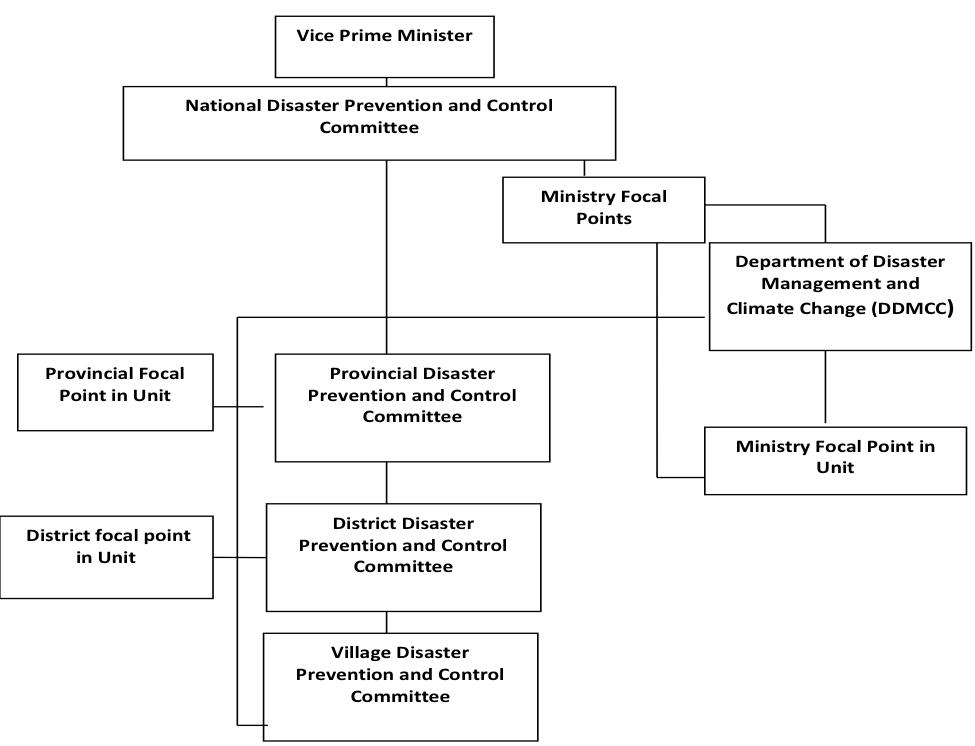
\includegraphics[width = \linewidth]{Figures/laopdr.png}
\end{center}
\end{figure}
   
{\flushleft \large \bfseries Lao Disaster Information System (LaoDi)}

\vspace{0.4 cm}

This initiative aims to strengthen the capacities of Lao PDR to provide information on disaster damage and loss to support national planning and Sendai1 framework. The LaoDi provides authorized users to access disaster data and enables to monitor, analyze vulnerabilities in specific area in Lao PDR and the collected data will be shared with line ministries and stakeholders.

\vspace{0.4 cm}

LaoDi was developed to record, store and analyze loss and damage data in Lao PDR. It was established by DDMCC with technical and financial support from the United Nations Development Programme (UNDP) and the Asian Development Bank (ADB). 

\vspace{0.4 cm}

LaoDi has two modules:  Administration and Analysis Module

\begin{enumerate}
\item Administration Module is designed for authorized user such administrator ora supper user. In this module, the user can (i) manage the database (add, update or delete); (ii) Manage region (provinces, districts and villages); (iii) Manage the  collected data(  delete, modify and updated); (iv) Manage  the maps and (v) Create and manage other users.
\item Analysis Module is for general users to access, the user can (i) analyze the collected data by queries; (ii) identify the  vulnerable area by  province, district  but not yet by villages or by village cluster; (iii) identify the  vulnerable areas by  causes,  type of disasters; and (iv) report  the analyzed result with graphs, tables and maps.
\end{enumerate}

LaoDi data can be exported to Microsoft Excel by statistics and crosstab statistics tools, while data analysis can be made using the chart and thematic map tool. Data analysis can be made at national level, provincial level, district level and village level from selections of query criteria. The LaoDi data is ongoing and will be updated by the Department of Disaster Management and Climate Change (DDMCC), Ministry of Natural Resources and Environment(MONRE). It is open and accessible to the general public at www.laodi.laodisaster.gov.la.

\vspace{0.4 cm}

The LaoDi online application used DesInventar methodology (www.desinventar.net). The database platform and methodology have been implemented in 25 countries in the Asia Pacific region, as well as America, Africa and Europe. LaoDi was established in Lao PDR by DDMCC after a series of consultation workshops between DDMCC officials and UNDP, followed by validation with key line ministries who will be provided data on disaster loss and damage.

\vspace{0.4 cm}

The LaoDi is focuses on direct loss and damage data resulting from natural disasters in Lao PDR, including human life, housing, road agriculture, and education and health sectors. The LaoDi data was collected from provincial disaster management committee (PDMC), district disaster management committees (DDMC), the Ministry of Agriculture and Forestry (MAF), Ministry of Public Works and Transport (MPWT), Ministry of Labor and Social Welfare(MLSW), Ministry of Health (MoH), Ministry of Education, and provincial departments of these line ministries.

\vspace{0.4 cm}

The data of loss and damage from natural disaster are primarily collected from Provincial Disaster Management Committee which also is focal point secretariat. However if the data is not available from PDMC, the data is based on following concerned ministries.

\begin{itemize}
\item Data of human life and housing is collected from Ministry of Labor and Social Welfare(MLSW)
\item Data road sectors is collected from Ministry of Pubic Work and Social Welfare(MPWT)
\item Data of agriculture is collected from Ministry of Agriculture and Forestry(MAF)
\item Data of hospital and health centers is collected from Ministry of Health(MH)
\item Data of schools is collected from Ministry of Education and Sports (MES).
\end{itemize}


{\flushleft \bfseries Current available data in LaoDi is}
\begin{itemize}
\item The  historical data between 1990 and 2012  received from Ministry of Labor and Social Welfare
\item Updated Data: from annual reports of DDMCC between 2014 and 2016.
\item Total of 4448 datacard(records): up to district level  with five main sectors(Agriculture , education, health, labour, and road sectors)
\item Only around 150 road-related data: roads and bridges  data
\item Only 50 data variables (data types): number  of  Deaths people; Injured people; Missing people; Destroyed houses; Destroyed crops; Damaged road; 16 main disaster events; Floods, drought, epitomic, cool wave....
\end{itemize}

{\flushleft \bfseries Expected data for LaoDi is}
\begin{itemize}
\item Direct disaster data  of five main sectors: (i) Agriculture sector; (ii) Education sector; (iii) Health sector; (iv) Labor and social sector and (v) Road sector;
\item Data variables will be more than 170 (e.g number of people deaths, destroyed house,…)
\item Main disaster events are around 20 (Floods, drought, epitomic, cool wave...)
\item The regularly up to-date data  will be received  from provinces via online data entry   and  up to villages level
\end{itemize}

\textbf{LaoDi is still operated offline, but work in Local Area Network (LAN) of the DDMCC office.}

\vspace{0.4 cm}

{\flushleft \bfseries Key Challenges}
\begin{itemize}
\item Lacking human capacity in the area of disaster risk management and emergency responses;
\item Information and data is not yet updated; 
\item Some data and information is not yet available;
\item Local Infrastructure to support geo-based infrastructure is still young; and 
\item Lacking investment.
\end{itemize}

\begin{center}
{(Kob Chai lai lai - Thank you very much) \par}
\vspace{0.5 cm}
\textbf{Keywords:} remote sensing, economic development, challenge, technology independence.
\end{center}

\section{Malaysia}

\vspace{0.5 cm}

{
	\begin{center}
	{\large \bfseries Geospatial Technologies in Malaysian Disaster Planning and Management\par}
	\vspace{0.5 cm}
	{\bfseries Associate Professor Sr Gs Dr Abdul Rashid Mohamed Shariff\par}
	{\itshape University Putra Malaysia\par}
	{\itshape Email: rashidpls@upm.edu.my\par}
	\end{center}
	{\tab The ASEAN Social-Cultural Community (ASCC) Blueprint 2015-20125 is an important step forward in creating a more resilient and self-sustainable community and region. This paper shares the Malaysian approach and hopes the cooperation and ASEAN spirit will lead to the materialization of this highly valued blueprint.
	
\vspace{0.4 cm}

The National Security Council is a Federal agency under the Prime Minister's Department mandated with the responsibility for managing and coordinating the implementation of policies related to the security of Malaysia and providing policies and mechanism for national disaster management and relief. The three core functions of the NSC are defending national sovereignty and strategic importance, crisis and disaster management and border management of land, maritime and air. In order to coordinate government agencies in tackling disasters, the National Disaster Management Agency (NADMA) was set up in 2015 and it coordinates the relevant authorities such as the Malaysian Armed Forces, Police, Malaysian Civil Defence Department, Fire and Rescue Department, Rela, Social Welfare Department and other relevant agencies. NADMA's GIS Centre at Cyberjaya  using the Dashboard Concept is expected to be operationalized in 2018 with Malaysian Space Agency (ANGKASA) providing the geospatial data processing infrastructure and support. The core agencies providing geospatial data for disaster management are Malaysian Metrological Department (MMD), National Survey and Mapping Department (JUPEM), National Remote Sensing Agency (ARSM), National Space Agency (ANGKASA), Malaysian Centre for Geospatial Data Infrastructure (MaCGDI), Public Works Department (JKR), Drainage and Irrigation Department (JPS). In keeping abreast with current developments, low-cost satellites are gaining interest, especially for environmental monitoring, particularly from a state government and university research centres. A framework of cooperation is being formalized for cooperation between Malaysian universities and ANGKASA  on satellite research and development, with a low cost micro-satellite program with Hokkaido/Tohoku university being planned. Research on Deep Learning and artificial intelligence (AI) has made a sound footing at local universities and there is good potential to develop application systems from current research level status. Big data holds a major potential to contribute to disaster management and the role of MacGDI to enable  data sharing and a free flow of data will enhance the useful applications of geospatial data. The national geospatial policy currently being formulated will catalyse this cooperation. The use of high precision satellite positioning will help in getting better mapping and location information for better disaster management decision making. Currently a high precision multi-gnss is being tested at an oil palm plantation with JAXA and collaboration with Keio university, Tokyo university and Universiti Putra Malaysia. The results of such collaboration will not only benefit agriculture but the resulting high accuracy maps can be of aid to disaster management, particularly in flood mitigation. In order to have greater acceptance of technology, the production of simple to operate and beneficial devises become necessary. Internet of Things (IoT) is one example of such developments which has received support of the Malaysian government. Plans are afoot to create an entrepreneurship industry in this field and Malaysian Institute of Microelectronics Systems (MIMOS) has been entrusted with this leadership role. Mimos has created a roadmap for the national IoT strategy (\url{http://mimos.my/iot/National_IoT_Strategic_Roadmap_Summary.pdf}). 
	
\vspace{0.4 cm}
  
The major cost component during the disaster management implementation is the logistics management that can make about 80\% of total cost of a disaster response. It is not only an  issue of cost but the need for timely and efficient coordination as disaster logistics management is currently being handled by multiple government organization with different objectives and stakeholders. Although each agency has a working logistics management system, there is no apparent communication with each other. There is no real-time system on the availability and current location of resources and assets that have been allocated for the purpose. Based on feedback from experienced ground personnel who has been involved in dozens of disaster operations, it was found at the 'de-brief session' that the main problems that exist and need to be addressed is the communications problem. The communication flaws can be contributed by the weaknesses among the personnel, the weaknesses of some agencies standard operating procedures (SOPs), command and order and from the radio emergency communication system itself.
	
\vspace{0.4 cm}
  
	Empowerment of local communities against natural hazards not only renders support to the disaster preventions efforts but when implemented as a WEB GIS, as in the case of Ulu Klang Highlands community, was found to have benefits of helping in the development of a community friendly web GIS based information system, ability to integrate the web site with data from metrological and other relevant sources, empowered the community to upload relevant environment sensitive information and to produce updated maps that can be printed and downloaded by local residents. These brought benefits to the residents as they were able to view and have easy access to the map in the web and other information which are relevant such as rainfall data, can be active players in monitoring their local topography an environment and can link directly to metrological and other external data sources.
		
\vspace{0.4 cm}
  
	Based on the assessment of the current situation, some potential projects that can benefit from the integrated use of the space and geospatial technologies are cross-boundary haze, illegal human trafficking, crowd sourcing information and Illegal land cutting and land clearing.
		
\vspace{0.4 cm}
  
	Although there is ASEAN cooperation and agreement on trans-boundary haze pollution, well integrated and efficiently executed geospatial applications will help in the success of combating trans-boundary haze, especially through effective data sharing procedures. Illegal human trafficking is a problem awaiting a geospatial solution. This activity is directly a geospatial phenomenon as no illegal human trafficking can occur without geographical movement of the victim. The current mobile telephone technology can be an innovative tool in helping trace this illegal human movement. As greater masses of people can exposed to technology the time is ripe to educate and cultivate crowd sourcing data from people on the ground. In the case of Malaysia, just the Civil Defence Agency alone has 1 million people who are their ground volunteers. Tools such as low cost high accuracy multi-gnss receivers will enable these volunteers to supply ground data with very high accuracy. As for land cutting and clearance activities, monitoring and enforcement of illegal and dangerous cutting and clearing of land can help avoid landslides, mud floods and related disasters which have brought catastrophic consequences in the past.
		
\vspace{0.4 cm}
  
In conclusions, it is indisputable that space and geospatial data is a critical requirement in building a resilient society. Use of these data, together with a data infrastructure and data sharing are fundamental  parts of a resilient system. Communication, training and retraining are vital components of capacity building that cannot be overlooked. With the current pace of technological changes, having a society that is up to date, knowledgeable and skilful in the use of the geospatial technology will be an asset to the country and ASEAN region. The wisdom and efficiency in utilizing these geospatial technology will ensure a safe and secure society for generations to come. 

\par}
}


\section{Myanmar}

\vspace{0.5 cm}

	\begin{center}
	{\large \bfseries Presentation Summary by Myanmar on the ERIA Research Project Wrap-up Meeting\par}
	\vspace{0.5 cm}
	{\bfseries Daw Thiri Maung\par}
	{\itshape Ministry of Social Welfare, Relief and Resettlement (Myanmar)\par}
	{\itshape July 6, 2017\par}
	\end{center}
	{\tab Myanmar is prone to the natural disasters and the frequencies and the intensities of the disasters are getting higher.  According to the global reports, the rank for the disaster frequency of Myanmar is 42 out of 171 countries while the rank for the readiness for response to the disaster is 15.
		
\vspace{0.4 cm}
  
After the catastrophic cyclone Nargis in 2008 which triggered the 21\% total damage and loss of GDP in 2007 fiscal year, Myanmar has made emphasis to the Disaster Risk Reduction in momentum. The country bears average annual loss of about 3\% of GDP due to the natural disaster. In 2015, it also suffered the nation-wide flood and severe landslide in the mountainous regions especially in the Western part of the country and these happened 3.1\% total damage and loss of GDP. The Government of Myanmar has laid down its development vision to be 'A developed nation (middle income country) that is integrated into the global community' in its National Comprehensive Development Plan (NCDP), 2030. A disaster can draw back the development gains and can interrupt the development and sustainability of the country. In this regards, to achieve the resilient development in Myanmar, the National Disaster Management Committee (NDMC) has been comprised and chaired by the Vice President of the Government of the Union of Myanmar aiming to promote the Disaster Management System in Myanmar in line with global and regional frameworks. 
		
\vspace{0.4 cm}
  
The NDMC is the highest decision making body and 12 working committees has been composed under the supervision of the NDMC. Relief and Resettlement Department (RRD) of the Ministry of Social Welfare, Relief and Resettlement is the focal department for the Disaster Management. Myanmar also enacted the Disaster Management Law (2013) and the Disaster Management Rules (2015) as law enforcement is necessary to ensure the sustainable development while carrying out the disaster risk reduction and management activities without any interruption. Moreover, Myanmar Government developed the Myanmar Action Plans on Disaster Risk Reduction-MAPDRR (2012) and now MAPDRR is under revision in line with SFDRR, SDGs and other regional and global concerned frameworks.
		
\vspace{0.4 cm}
  
Based on the experience and lesson-learnt from the previous MAPDRR (2012), the new MAPDRR (2017) will be comprised with four main areas and one of them is "Assessing disaster and extreme events risk and creating public awareness on DRR in Myanmar" and there will be 8 priority actions for risk reduction by mainly applying the space-based and geospatial  technologies. 
		
\vspace{0.4 cm}
  
Since 2012, Myanmar has started to upgrade its disaster management system by utilizing advanced technology like space technology and received the Technical Advisory Mission (TAM) of the UNSPIDER of UNOOSA. The TAM provided the recommendations to utilize the space technology widely in the disaster management. Myanmar Government has understand that the advanced and techanical based disaster management mechanism has become the crucial and necessary requirement for attempting to have the resilient community to the natural disaster and sustainable development and RRD reformed its organization structure by means of the establishment of the Emergency Operations Centre (EOC) as one of the operating organs of RRD in 2013. EOC has been comprised with four different units including the technical unit for handling the space-based and geospatial information. This technical unit is still under nurturing stage for the human resource development to get fully functioning for analysing the satellite imageries and perform the researches on the risk analysis to contribute for the disaster management activities. It is still necessary to get the capacity development measures for the technical skills improvement and experiences as well.
		
\vspace{0.4 cm}
  
Myanmar also tried to be a member to the International communities for utilization of space technology in disaster emergency and disaster management and already got the technical assistance and data and information in disaster emergency from the Sentinel Asia and the International Charter. Being a member to the Asian Disaster Reduction Centre (ADRC), Myanmar has the rights to request to the Sentinel Asia. Moreover, Relief and Resettlement Department (RRD), the National Disaster Management Organization (NDMO) has become the Authorized User of the International Charter to get the speedy activation process. Besides, Myanmar has another option for accessing the Space technology that is the Procedural guidelines on "Utilization of Earth observation data during emergency response" developed for ASEAN group.
		
\vspace{0.4 cm}
  
Furthermore, RRD is tried to allocate the budget for purchasing the high resolution satellite imageries in the future fiscal year for having the chance to utilize the satellite imageries in the relocation stage after some disaster emergencies and risk assessment measures when it is necessary to provide the said images. In addition, the training course for the Geoinformatics Applications in Disaster Management was developed and this course is used to deliver in the Disaster Management Training Centre (DMTC) of RRD to the government officials and staffs who are responsible to the disaster management in Myanmar. The objective of the training is to "raise awareness amongst the participants and develop basic skills for effectively utilising the Geographic Information Systems and RS/ space based information in Disaster Management". This course is comprised with 4 modules, namely; Disaster Management Terminologies and Concepts, Introduction to GIS, Remote Sensing, GPS and Internet Mapping Services, Geoinformatics for Mapping and monitoring of Hazards, Vulnerability and Risk Assessment and Geoinformatics for Disaster Management Planning and Emergency Response.
		
\vspace{0.4 cm}
  
Disaster risk reduction and disaster management is the cross-cutting issue and it is very crucial for the national development and sustainability. In order to ensure the sustainable development, it is vital to be disaster resilient and the disaster risk reduction measures are critical to make the best use of space-based and geospatial technologies. Moreover, it is important to dessiminate the results and products acquired from these technologies not only to the concerned agencies to have the practice to utilize in their routine works in DRR but also to the communities for their awareness raising. Exchanging the knowledges and best practices on utilization of space-based and geospatial technologies through the regional and global meetings and workshops are very helpful to widely utilze and apply the technologies in the field of disaster management.
\par}


\section{Philippines}

\vspace{0.5 cm}

	\begin{center}
	{\large \bfseries Disaster Risk Reduction and Management (DRRM) in the Philippines and the Southeast Asian Region through 
Space Technology\par}
	\vspace{0.5 cm}
	{\bfseries Adrian Josele G. Quional\par}
	{\itshape National SPACE Development Program\par}
	{\itshape 37th Flr. LKG Tower, 6801 Ayala Ave., Makati City, 1226 Philippines\par}
	\end{center}
	{\tab The Philippines is located near the equator and along the Pacific Ring of Fire which makes it vulnerable to natural disasters such as typhoons, earthquakes, and volcanic eruptions, endangering the natural resources and biodiversity endowed to the country. A notable major disaster that struck the Philippines is Typhoon Haiyan (local name: Typhoon Yolanda) on November 2013 which brought an estimated cost of damages worth PHP 89.6 billion (USD 1.77 billion), with 6,300 deaths and 1,081 gone missing. This scenario is a major concern for the Philippines and measures needed to be adapted given that a similar disaster is possible to happen in the future due to the Philippines' location. An effective Disaster Risk Reduction and Management (DRRM) measure that can be taken by the country is the use of space technology, particularly satellite technology.
		
\vspace{0.4 cm}
  
The country is gradually emerging as a space-faring nation, as evidenced by the continuous space development efforts throughout the past years. Looking ahead, the Philippines, through the National Space Promotion, Awareness, and Capabilities Enhancement (SPACE) Development Program (or NSDP), developed strategic roadmaps for the future space program of the country. Among these roadmaps includes the Satellite Development Roadmap which contains the satellite requirements of the Philippines for the next 15 years. Particularly, satellite technology for the Philippines would bring enormous benefits for the country, particularly on applications for national security, agriculture, and disaster management. While all of the satellites being planned by the Philippines have a direct or indirect application for disaster management (in terms of communications and Earth observation applications), there are particular satellites that has the greatest contribution to this use. In particular, planned satellites that have immense applications for disaster management includes a Synthetic Aperture Radar (SAR) satellite and a Microwave Satellite for Precipitation Monitoring. 
		
\vspace{0.4 cm}
  
The coupled use of a SAR and a Microwave Satellite can greatly enhance DRRM efforts throughout the country. By measuring precipitation and rainfall using a Microwave Satellite, combined with the data from the SAR satellite, comprehensive results can be timely distributed to various decision and policy makers in critical times of disasters; thereby enhancing humanitarian aid for the affected areas.
		
\vspace{0.4 cm}
  
Given this strategic plan of the country to develop satellites for disaster management, the Philippines can lead the way for the Southeast Asian Region, being in a prominent location for typhoons and disasters. As the country is strategically located between the Pacific Ocean and the mainland Southeast Asia, the path of typhoons mostly cross the Philippine archipelago onto either East Asia or Southeast Asia, making the country, indeed, at the forefront of typhoons. Therefore, being at the frontlines of Southeast Asia in terms of typhoons, an effective utilization of satellite technology for disaster management in the country would help the whole region as it would reduce the risk of disaster for the other countries. An "ASEAN Satellite Constellation" of SAR and/or Microwave Satellites would prove a valuable asset for the region as it would mean a greater regional coverage.
		
\vspace{0.4 cm}
  
However, physical infrastructure for satellite technology would not be effective without satellite information sharing. Thus, there is a need for the countries in the region to engage in satellite information sharing to promote inter-operability and interconnectivity throughout the region in terms of satellite technology. A Satellite Data Sharing Policy for the Southeast Asian Region for disaster management, amenable to each country's policies and not endangering the security of each nation, would prove useful.
		
\vspace{0.4 cm}
  
Lastly, a Regional Center for Water Information can be established in the Philippines to pool in researchers and technologists from Southeast Asia and to facilitate satellite data sharing among countries. This Regional Center can be the centerpiece in Southeast Asia in terms of utilizing water information, in this case for disaster management. 
		
\vspace{0.4 cm}
  
The Philippines has been at the forefront of disasters and typhoons in Southeast Asia, as manifested by the recent Typhoon Haiyan that struck the Philippines on 2013, where no other typhoon to date matches the devastation brought upon by it. With the Philippines slowly emerging as a space-faring nation, crafted plans for its future space program, the development and utilization of various satellites for disaster management is included at the forefront of its strategy. The use of a SAR and Microwave Satellite, not only in the Philippines but also for the whole Southeast Asia, would be a valuable asset. A Satellite Data Sharing Policy for the region should also be discussed upon in order to effectively utilize the satellite data. Lastly, a Regional Center for Water Information can be established in the Philippines which would play a vital role in the region in the facilitation of water information and research. 
\par}

\section{Thailand}

\vspace{0.5 cm}

{
	\begin{center}
	{\large \bfseries Thailand Disaster Risk Manage utilized Space Technology\par}
	\vspace{0.5 cm}
	{\bfseries Jakrapong  Tawala\par}
	{\itshape Geoinfomatics and outreach scientist\par}
	{\itshape Geo-informatics and Space Technology Agency (Public Organization)\par}
	{\itshape 196 Phahonyothin Rd., Ladyao, Chatuchak, Bangkok, THAILAND\par}
	{\itshape jakrapong@gistda.or.th\par}
	\end{center}
	{\tab Thailand is less susceptible to natural hazards than many of the countries in the Asia – Pacific. Geography and location of Thailand help insulate the country from many of the impact of metrological and geophysical natural disasters. However, Thailand is agricultural industry and highly development urban areas leave large portions of the population and the economy vulnerable to disasters such as flooding, drought, landslides and forest fire. 
	
\vspace{0.4 cm}

Over the past two decades, space technology has become a significant part of our daily lives and can play important roles in the disasters risk reduction and management. Thailand has been involved in satellite remote sensing since the launch of NASA ERTS-1 Programme in 1971 through Thailand Remote Sensing Programme (TRSP) under the National Research Council of Thailand (NRCT). In 2000, Geo-Informatics and Space Technology Development Agency (Public Organization): GISTDA was established in order to enhance the utilization in remote sensing and GIS and responsibilities the activities for space technology applications in Thailand particularly for disaster management. Thailand Monitoring System (TMS) was initiated by GISTDA to cope and monitor disaster and daily on-line publish analytic geo-information from satellite imagery for related organization and private sector. The system includes flood, drought and forest fire and can be accessed at tms.gistda.or.th.

\vspace{0.4 cm}

Flooding is the most serious hazard in Thailand and every part of the country struggles with flood-related damages annually.  During monsoon season in Thailand, GISTDA monitors flood situation and agricultural areas in Thailand every 7 days utilized RADARSAT data to monitor agricultural areas and evaluate damaged zones for general areas and Cosmo-skymed data to monitor critical areas due to its constellation capability (4 satellites). Rain cloud information from COMS satellite is available in hourly, daily, weekly and monthly. These information are served to the government and published via web service (flood.gistda.or.th)

\vspace{0.4 cm}

Drought is an increasingly serious hazard for parts of central and eastern of Thailand. Drought conditions are most common from January through May and are alleviated by the onset of monsoon season. GISTDA use a set of MODIS data (7 days) to calculate drought indices, Normalized Difference Vegetation Index: NDVI and Normalized Difference Water Index: NDWI, for drought risk area assessment and weekly published on http://drought.gistda.or.th. This information is necessary for the government to warn and assist the farmer. Moreover, surface water database from Landsat satellite image has been collected for drought monitoring as it is an indicator of water shortage. GISTDA also developed Field Server Ground Station to automatics collect field data such as humidity, soil moisture, rain volume and crop growing etc. This data will be integrated with satellite data for precise data from the field. Currently, there are 25 stations was installed spread the whole country in difference crop type. 

\vspace{0.4 cm}

Forest Fire annually occurs during the dry season from December to May with their peak in February-March. Fires, Mostly classified as surface fires, mainly take place in; Mixed Deciduous Forest, Dry Dipterocarp Forest, and Forest Plantations, and to some extent in Dry Evergreen Forest, Hill Evergreen Forest or event in some parts of the Tropical Rain Forest. These surface fires consume surface litter, other loose debris on the forest floor and small vegetation. In Thailand, forest fire is daily report TMS system (fire.gistda.or.th) publishing daily hotspots utilized TERRA/AQUA-MODIS data, haze, smoke. GISTDA weekly generates wildfire risk area analyzed from hotspots accumulated 10 years , land-use, burnt NDWI area and weather to predict trend of fire in each year. Burnt area every 16 days also extracted using LANDSAT- 8 satellite image. Beside, GISTDA established GISTDA Forest Fire and Smoke Operation Center in 9 provinces in northern of Thailand where forest fire is common issue.   In this center will received product of remote sensing and GIS data from GISTDA to support forest fire management and training of data interpretation and effectively using form GISTDA experts. Currently, GISTDA receives daily hotspot data from SUOMI-NPP satellite (2 time/day) integrate with MODIS data. By doing this, Thailand will have more detail information of forest fire and number of hot spot may significantly increase because number of round and resolution of satellite. Mobile Application for alert and report the situation in the fire area was developed to get more precise fire location data. 

\vspace{0.4 cm}

Base on GISTDA experiences, space technology still remain plays important roles for disaster management in every state of disaster situation in the future.  Satellite image gives the overview information of disaster situation which necessary for understanding, management and decision making. Precise location information form constellation of GNSS will lead you to exact location to rescue and assist on time. Right information integrate with appropriated management processing and new technology will result rapid resolved situation for example hot spot situation in northern part of Thailand has continued to decline in every year because of management in the right point and location with understanding the situation utilized information from space technology. 
\par}
\begin{center}
\textbf{Keywords:} space, technology, natural disasters, Thailand \par
\end{center}
}

\section{Vietnam}

\vspace{0.5 cm}

	\begin{center}
	{\large \bfseries Potential of GeoSpatial/Space -- Based Service in Vietnam\par}
	\vspace{0.5 cm}
	{\bfseries Dr. Vu Anh TUAN\par}
	{\itshape Vietnam National Satellite Center\par}
	\end{center}
	{\tab The 2016 World Disaster Report showed that Vietnam has been one of five countries most affected by the natural disaster and climate change in the world. In the last 10 years, according to MONRE (Ministry of Natural Resource and Environment), there are around 500 deceases, damage of 1.5\% of GDP per year cause by disasters. There are many type of disaster in Vietnam.  The top five high frequency disasters are: Flooding; Storm; Draught; Flash Flooding; Erosion/sedimentation.
	
	
Using Space-based service for disaster management in Vietnam is currently issues by research institutions as well as management agencies. Recently, Vietnam is building up an infrastructure for geospatial data called Vietnam Data Cube. This will be open-sharing system for all available geospatial data of Vietnam, including free satellite data such as Landsat, MODIS, Sentinel; Vietnam's satellite data (VNREDSat 1; LOTUSat 1 and 2) and other data. The Vietnam Data Cube is being built based on the Data cube (http://ceos-cube.org/). The Vietnam Data Cube will provide ability of ease of use and access to space-based data with multiple dataset interoperability and spatial consistency. It is also combined with built-in data processing algorithm and API which can be used for "Analysis Ready" of data products for all users. The Vietnam Data Cube is planned to be launched in January 2018 with two demonstrate applications: Forest monitoring and Water quality monitoring. Since the open of space-based data and service of Vietnam Data Cube, it can be considered for nominee of space-based service for disaster management in Vietnam as well as in ASEAN countries. However, toward a space-based service for disaster management, the investment issues need to be clarified are: infrastructure (Data Cube – based); Data system (Data Cube similar); Software; Trained professionals and Web-based services system. This system will help ASEAN countries to share common understanding, EO and GeoSpatial data and help people in early warning; rescue information.
\par}
